\section{CST Model and Simulation Method}
\label{sec:model-and-method}

The CST model consists of an input air region, a parameterized dielectric slab, and an
output air region. Geometry is defined in millimeters and frequency in GHz. The
frequency-domain solver evaluates the structure up to 1~GHz, with electric- and
magnetic-field monitors at 1~GHz.

\subsection{Geometry and Material Parameterization}

The principal dimensions are
\begin{equation}
H_0=44.87~\text{mm},
\qquad
W_0=299.79~\text{mm},
\qquad
L_0=299.79~\text{mm}.
\end{equation}
The slab thickness is $L_0$, approximately one free-space wavelength at 1~GHz.
The dielectric relative permittivity is controlled by the CST parameter
\texttt{eps}; the outer regions are vacuum.

\begin{figure}[H]
    \centering
    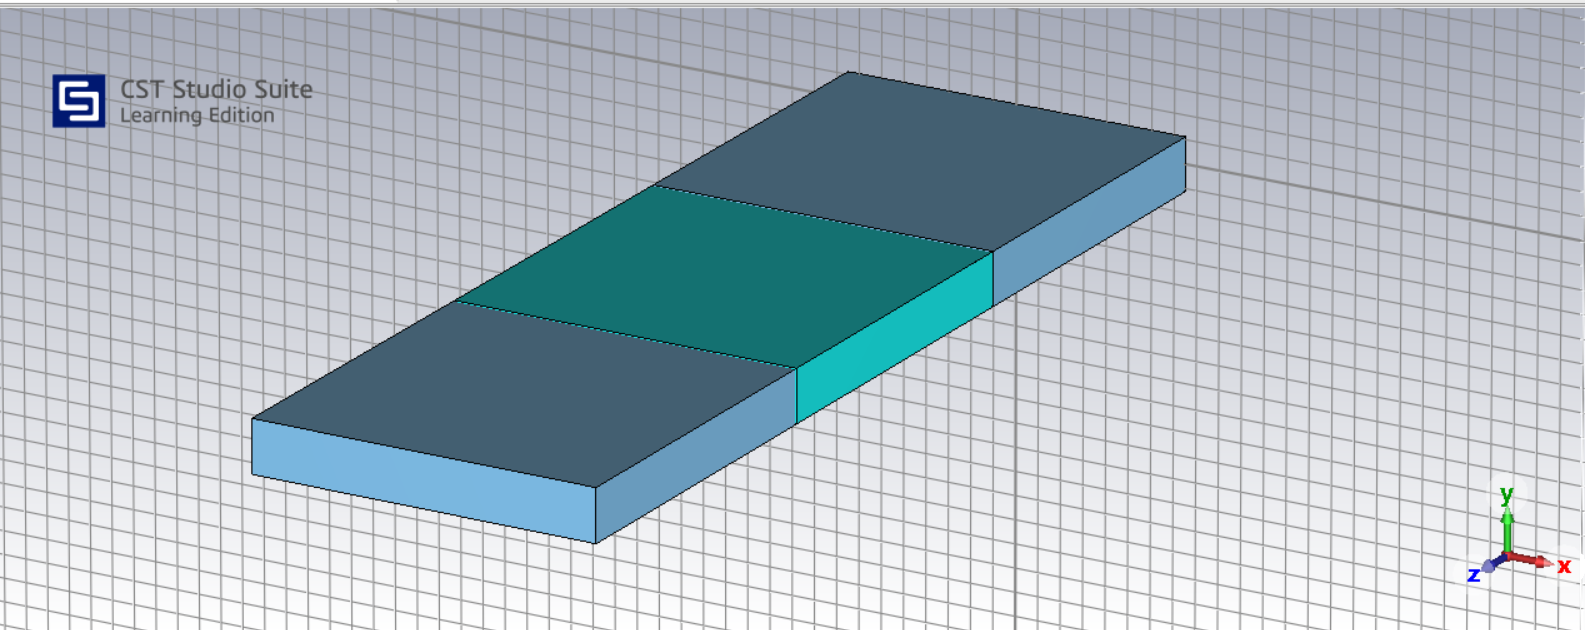
\includegraphics[width=0.82\textwidth]{figures/cst_results/Fig_geometry.png}
    \caption{Preserved CST geometry of the air--dielectric--air structure. The center
    brick is the parameterized dielectric slab.}
    \label{fig:geometry}
\end{figure}

\subsection{Boundary Conditions}

Electric boundaries are applied to the two $x$-normal side faces and magnetic
boundaries to the two $y$-normal side faces. The two longitudinal $z$ faces are open.
Together, the paired electric and magnetic walls create a TEM-like propagation
environment in the finite transverse model.

\begin{figure}[H]
    \centering
    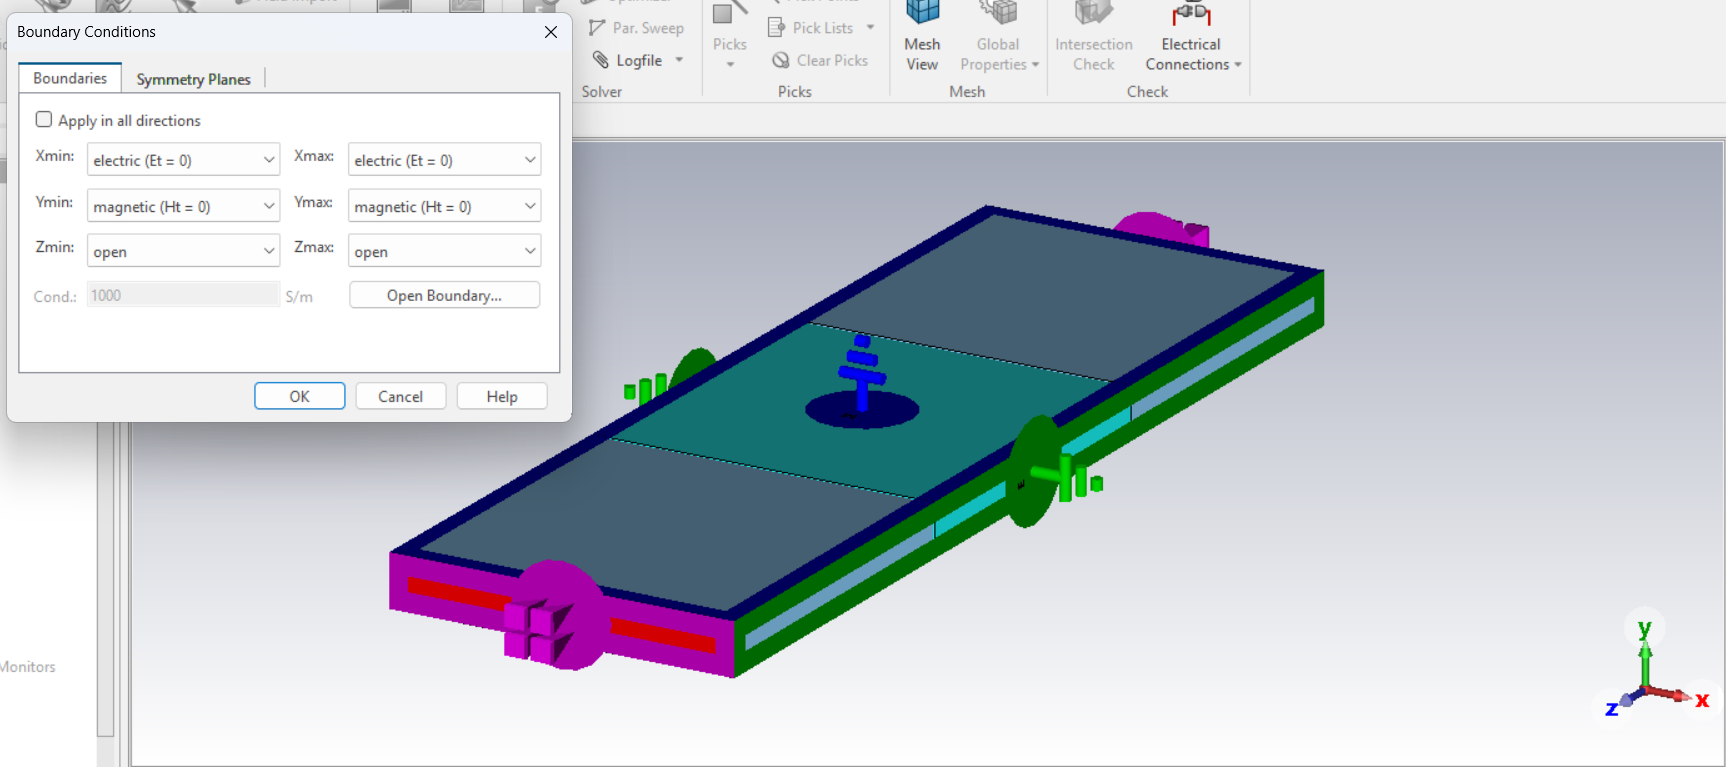
\includegraphics[width=0.82\textwidth]{figures/cst_results/Fig_boundaries.png}
    \caption{Preserved CST boundary-condition definition.}
    \label{fig:boundaries}
\end{figure}

\subsection{Ports and Modes}

Two waveguide ports are placed at the longitudinal ends of the model. The source report
states that one propagating mode was initially insufficient and that three modes were
requested at each port. The primary metric remains the fundamental-mode reflection
coefficient $S_{1(1),1(1)}$, denoted $S_{11}$ in the public report.

\begin{figure}[H]
    \centering
    \begin{subfigure}[t]{0.48\textwidth}
        \centering
        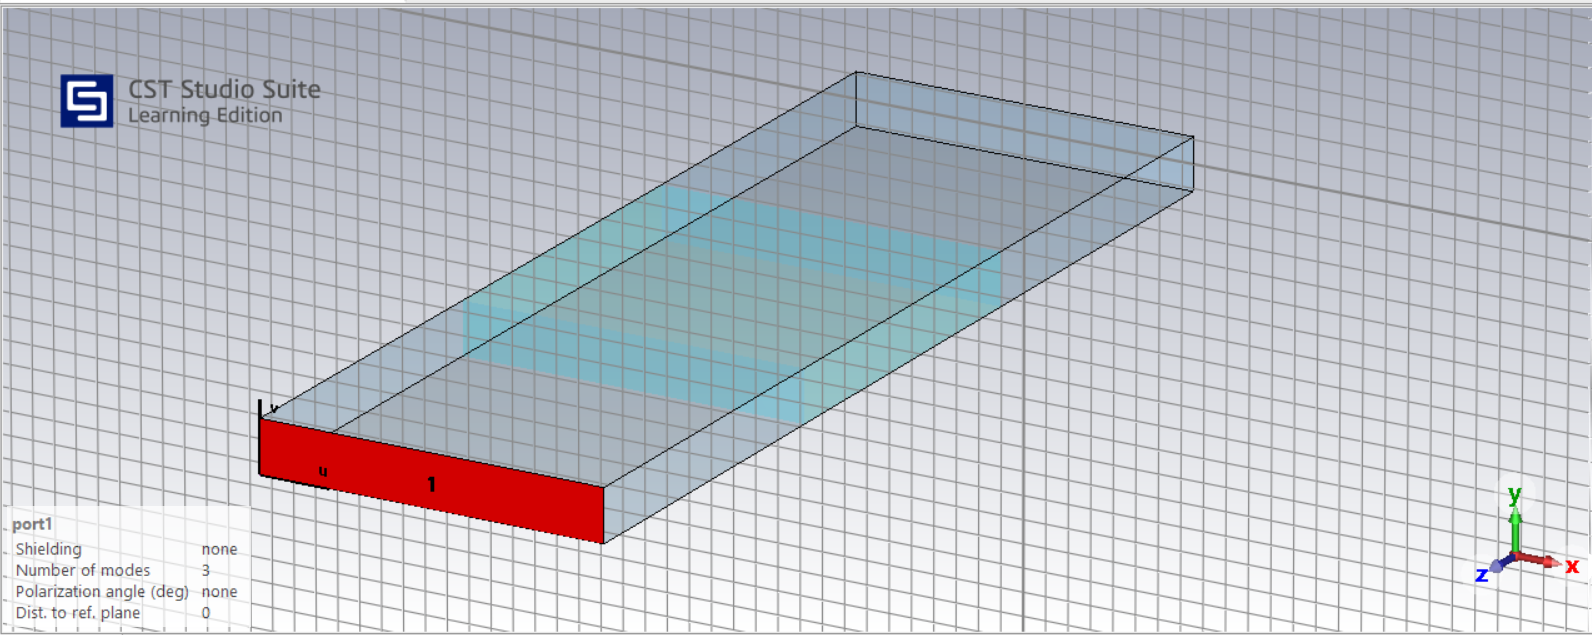
\includegraphics[width=\textwidth]{figures/cst_results/Fig_port1.png}
        \caption{Port 1.}
        \label{fig:port1}
    \end{subfigure}
    \hfill
    \begin{subfigure}[t]{0.48\textwidth}
        \centering
        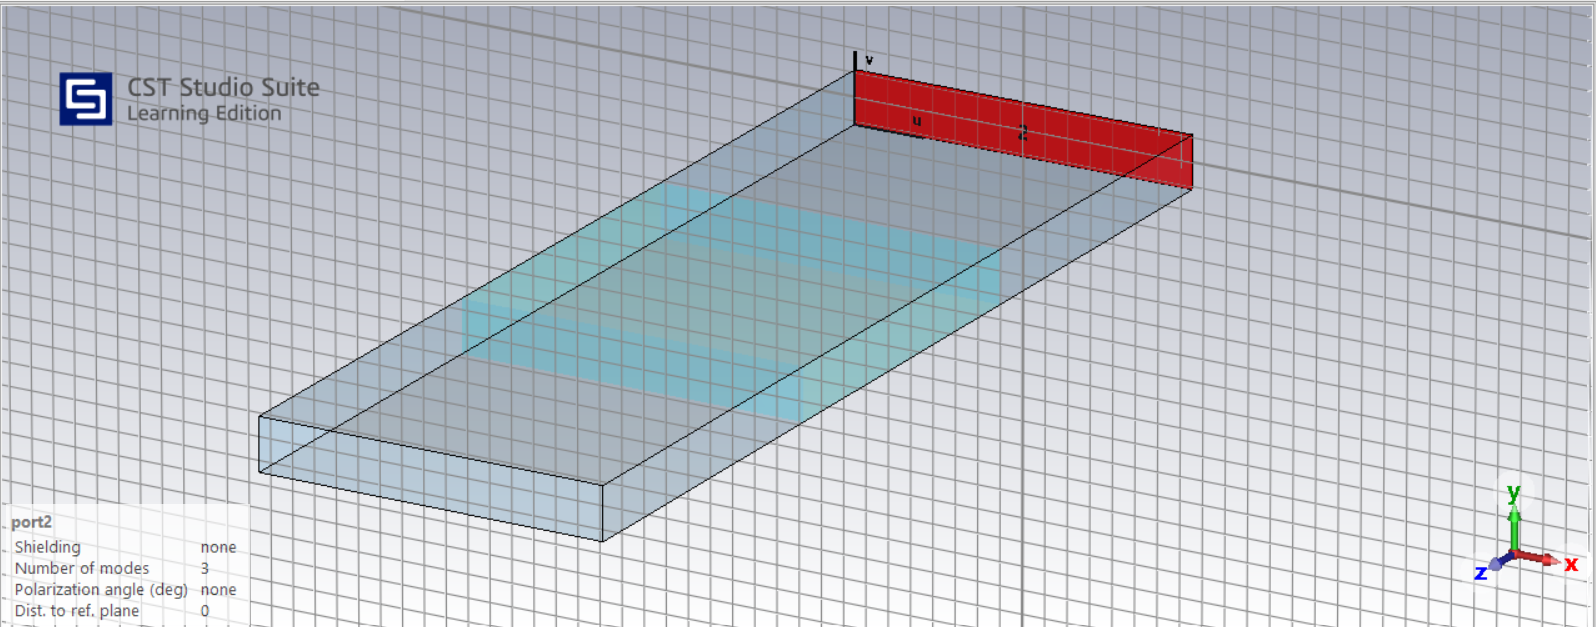
\includegraphics[width=\textwidth]{figures/cst_results/Fig_port2.png}
        \caption{Port 2.}
        \label{fig:port2}
    \end{subfigure}
    \caption{Preserved CST waveguide-port definitions.}
    \label{fig:ports}
\end{figure}

\subsection{Permittivity Sweep}

The parameter \texttt{eps} is swept linearly from 1 to 10 using 37 points, corresponding
to a 0.25 increment. The $S_{11}$ magnitude and phase are extracted at 1~GHz.

\begin{figure}[H]
    \centering
    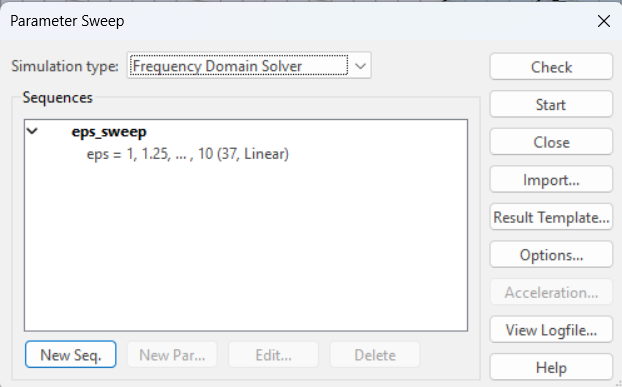
\includegraphics[width=0.70\textwidth]{figures/cst_results/Fig_parameter_sweep.png}
    \caption{CST parameter-sweep definition for relative permittivity.}
    \label{fig:parameter-sweep}
\end{figure}
